\chapter{\red{基礎理論と}従来手法}
\label{chap:conv}

%----------------------------------------------
\section{まえがき}
%----------------------------------------------
\red{本章では,音源分離技術において必要となる手法の基礎理論とこれまでに提案されてきた音源分離手法について述べる.}まず,\ref{sec:ica}節では,提案手法の基礎理論となる音源分離手法のICAについて説明する.
\ref{sec:stft}節では,音響信号処理でよく用いられる,短時間フーリエ変換(short-time Fourier transform: STFT)について説明する.
\ref{sec:formularization}節では,時間周波数領域における音源信号及びBSSの定式化を導入し,\red{\ref{sec:fdica}節以降は,定式化したものを用いて説明する.}
\ref{sec:fdica}節では,\red{時間周波数領域で周波数毎にICAを適用する}FDICAについて説明する.
\ref{sec:pp}節では,\red{本提案手法の解決すべき課題である}パーミュテーション問題と呼ばれるFDICAに伴う問題の説明と,既存のパーミュテーション解決法について説明する.
\ref{sec:ivailrma}節では,パーミュテーション問題を回避するような音源分離手法であるIVA及びILRMAについて詳細を述べる.
\ref{sec:DNNs}節では,\red{本提案手法と既存のDNNに基づく手法の違いを理解するために,}既存のDNNを用いたパーミュテーション解決法について説明する.
\red{\ref{sec:conclu}節では,本章のまとめを述べる.}

%----------------------------------------------
\section{ICAの基本原理}
\label{sec:ica}
%----------------------------------------------
%----------------------------------------------

\red{本章では,BSSの基礎であるICA~\cite{ICA}について説明する.
なお,本章の説明では簡単のために,音源数及びマイクロホン数がいずれも2の場合を例として説明するが,本章記載の基本原理は音源数及びマイクロホン数がいずれも3以上の場合についても,一般性を失うことなく同様に説明できる.
但し,後述の通り,音源数とマイクロホン数は常に等しいという仮定が必要である.BSSの文脈では,このような「音源数がマイクロホン数以下」という条件を優決定条件と呼ぶ.}
\subsection{信号源の混合モデルと分離方法}
%----------------------------------------------
\blue{本項では,BSSの基礎であるICAについて説明する.}
今,2つの信号源$s_1(l)$及び$s_2(l)$があり,その混合信号を2つのマイクロホンで観測するという状況を考える.
ここで,$l = 1, 2, \cdots , L$は離散時間インデクスを示す.
マイクロホンで観測された信号を
$x_1(l)$及び$x_2(l)$とすると,2つの信号源の混合現象は次の連立方程式でモデル化できる.
\begin{eqnarray}
  \begin{cases}
    x_1(l) = a_{11}s_1(l) + a_{12}s_2(l)  \label{f:a1}\\
    x_2(l) = a_{21}s_1(l) + a_{22}s_2(l)  \label{f:a2}
  \end{cases}
\end{eqnarray}
ここで,信号の伝搬を表す係数$a_{mn}$は,時刻\blue{{$t$}}\red{$l$}には依存せず常に一定であると仮定する.
即ち,信号源の位置及びマイクロホンの位置が動かないことを仮定している.
また,$n = 1, 2, \cdots , N$,及び$m =
1, 2, \cdots , M $はそれぞ\red{れ}音源及びチャネルのインデクスを示す.
伝搬係数$a_{mn}$をまとめた行列を以下のように定義する.
\begin{align}
    \bm{A} = \red{\begin{bmatrix}
    a_{11}  & a_{12}  \\
    a_{21}  & a_{22}  \\
    \end{bmatrix}}
\end{align}
この行列$\bm{A}$は混合行列と呼ばれる.
観測信号ベクトル$\bm{x}(l) = \cancel{(x_1(l),x_2(l))^T} \red{[x_1(l),x_2(l)]^\mathrm{T}}$
信号源ベクトル$\bm{s}(l) = \cancel{(s_1(l),s_2(l))^T} \red{[s_1(l),s_2(l)]^\mathrm{T}}$
及び混合行列$\bm{A}$を用いて,式(\ref{f:a1})及び(\ref{f:a2})の連立方程式は次式のように書き直せる.
\begin{align}
    \bm{x}(l) = \bm{A}\bm{s}(l) \label{f:x}
\end{align}
ここで,$\cdot^\mathrm{T}$ はベクトルや行列の転置を表す.
分離信号を$\bm{y}(l) = \cancel{(y_1(l),y_2(l))^T} \red{[y_1(l),y_2(l)]^\mathrm{T}}$,分離行列を$\bm{W}$とそれぞれ定義すると,音源分離は以下のように表される.
\begin{align}
    \bm{y}(l) = \bm{W}\bm{x}(l)
\end{align}
このとき,混合行列$\bm{A}$の逆行列が存在する($\bm{A}$が正則)ならば,$\bm{W}=\bm{A}^{-1}$となるように$\bm{W}$を\blue{選択}\red{推定}することで,信号源$\bm{s}(l)$を推定することができる.
\begin{align}
    \bm{y}(l) &= \bm{W}\bm{x}(l)\\
    &= \bm{A}^{-1}\bm{x}(l)\\
    &= \bm{A}^{-1}\bm{A}\bm{s}(l)\\
    &= \bm{s}(l)
\end{align}

このように,混合行列$\bm{A}$の逆行列\red{である分離行列$\bm{W}$}を推定することで,音源分離を達成することができる.
しかしながら,音源やマイクロホンの位置関係が未知であるBSSにおいては,混合行列$\bm{A}$もまた未知である.
そこで,ICAでは,信号源の混合モデル式(\ref{f:x})の仮定の他に,信号そのものの統計的なモデル($p(s_1)$ 及び$p(s_2)$に対する仮定)を導入することで,分離\blue{フィルタ}\red{行列}$\bm{W}$を推定する.

%--------------------------------------------
\subsection{統計的独立性}
%----------------------------------------------
ICA による信号源分離を理解する上での重要な概念として,統計的独立性がある.
今,信号源$s_1(l)$及び$s_2(l)$を確率変数として扱い,それらの生成モデルを$p(s_1)$及び$p(s_2)$と定義する.
通常,各信号源($s_1(l)$及び$s_2(l)$)は互いに無関係であり,\red{例えば}$s_1(l)$から$s_2(l)$を\blue{推定}\red{予測や説明}することはできないはずである.
そのため,$s_1(l)$と$s_2(l)$は互いに統計的に独立とみなすことができ,次式が成立する.
\begin{align}
    p(s_1,s_2) = p(s_1)p(s_2) \label{f:s}
\end{align}
同様に,理想的な分離フィルタが推定できれば,分離信号$y_n(l)$も統計的に独立であるため,次式が成立する.
\begin{align}
    p(y_1,y_2) = p(y_1)p(y_2) \label{f:y}
\end{align}
ここで,$p(y_1)$及び$p(y_2)$はそれぞれ分離信号$y_1(l)$及び$y_2(l) $の生成モデルであり,$p(y_1, y_2)$は同
時分布である.
従ってICAによるBSSは,式(\blue{{\ref{f:s}}} \red{\ref{f:y}})が成立するような分離フィルタ$\bm{W}$を推定する問題であると解釈できる.
上記の問題を定式化すると,次式のように書き表せる.
\begin{align}
   \argmin_{\bm{W}}~ \mathfrak{I}(\bm{W})
\end{align}
\begin{align}
 \mathfrak{I}(\bm{W}) = \mathfrak{D}_{\cancel{KL} \red{\mathrm{KL}}}[p(y_1,y_2)||p(y_1)p(y_2)] \label{f:cost}
\end{align}
ここで,$\mathfrak{D}_{\cancel{KL} \red{\mathrm{KL}}}[p(s)||q(s)]$はカルバックライブラ・ダイバージェンス(Kullback--Leibler divergence: KL divergence)と呼ばれ,2つの分布間($p(s)$及び$q(s)$)の距離を測る関数として次式のように定義される.
\begin{align}
\mathfrak{D}_{\cancel{KL} \red{\mathrm{KL}}}[p(s)||q(s)] = \int{p(s){\rm log}~\frac{p(s)}{q(s)}}ds \label{f:kld}
\end{align}
また,分離\blue{フィルタ}\red{行列}$\bm{W}$で\red{観測信号を}線形変換する前($\bm{x}$)と後($\bm{y}$)の確率変数を考えたとき,それぞれ
の同時分布$p(\bm{y}) = p(\cancel{y1,y2} \red{y_1,y_2}) $と$p(\bm{x}) = p(\cancel{x1,x2} \red{x_1,x_2})$の間には,次式が成立する.
\begin{align}
    p(\bm{y}) = \frac{1}{|\mathrm{det}~\bm{W}|}p(\bm{x}) \label{f:detw}
\end{align}
式(\ref{f:kld})及び(\ref{f:detw})を用いて式(\ref{f:cost})を変形すると,最終的な最小化関数$\mathfrak{I}(\bm{W})$は以下のように書ける.
\begin{align}
\begin{split}
  \mathfrak{I}(\bm{W}) &= \int_{-\infty}^{\infty} \int_{-\infty}^{\infty} p(x_1,x_2){\rm log}~p(x_1,x_2)dx_1 dx_2 - {\rm log}~|\mathrm{det}~\bm{W}|\\
  &\quad -\int_{-\infty}^{\infty} p(y_1){\rm log}~p(y_1)dy_1 - \int_{-\infty}^{\infty} p(y_2){\rm log}~p(y_2)dy_2    \label{f:newcost}
\end{split}
\end{align}
ICAでは,式(\ref{f:newcost})\red{が最小化される分離行列$\bm{W}$を求めることで}\blue{を{$\bm{W}$}について最小化することで},信号源を分離する.

%----------------------------------------------
\subsection{\red{ICAにおける任意性}}
\label{subsec:ica_voluntariness}
%----------------------------------------------
\red{前項より,$y_{1}(l)$と$y_{2}(l)$の独立性を最大化する分離行列$\bm{W}$を求めるICAの最適化問題が定式化される.
しかしながら,分離信号の順序及びスケール(大きさ)の違いは,独立性の尺度である式(\ref{f:cost})に影響を与えないことは明らかである.
従って,ICAによって推定される分離信号$y_{1}(l)$及び$y_{2}(l)$には,以下の任意性が存在する.
%%%%%%%%%%%%%%%%%%%%%%%%%%%%
\begin{figure}[t]
    \begin{center}
        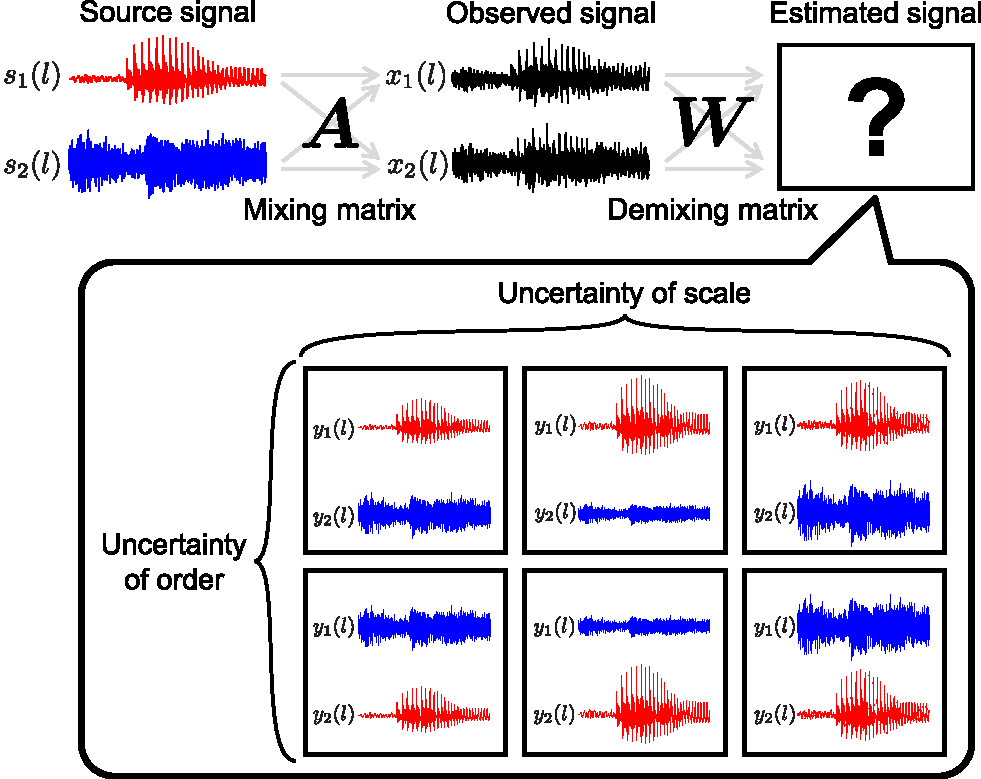
\includegraphics[width=0.95\columnwidth]{figures/uncertainty_ica.pdf}
    \end{center}
    \vspace{-8pt}
	\caption{Uncertainty in ICA. ICA cannot determine order and scales of estimated signals.}
	\label{fig:uncertainty_ica}
\end{figure}
%%%%%%%%%%%%%%%%%%%%%%%%%%%%
\begin{enumerate}
    \renewcommand{\labelenumi}{(\alph{enumi})}
        \item \red{分離信号の順序には任意性がある}
        \item \red{分離信号のスケールには任意性がある}
\end{enumerate}
これらの任意性は分離信号に対してFig.~\ref{fig:uncertainty_ica}のように現れる.
上記の任意性1より,元々の信号源の順序が入れ替わる可能性がある.また,任意性2より,分離信号のスケールが混合前の音源信号のスケールから変化してしまう可能性がある.
なお,信号のスケールの任意性に関しては,プロジェクションバック(projection back:~PB)法\cite{Matsuoka2001_PB}と呼ばれる補正方法が提案されている.
}

%----------------------------------------------
\section{STFT}
\label{sec:stft}
%----------------------------------------------
%%%%%%%%%%%%%%%%%%%%%%%%%%%%
\begin{figure}[t]
    \begin{center}
        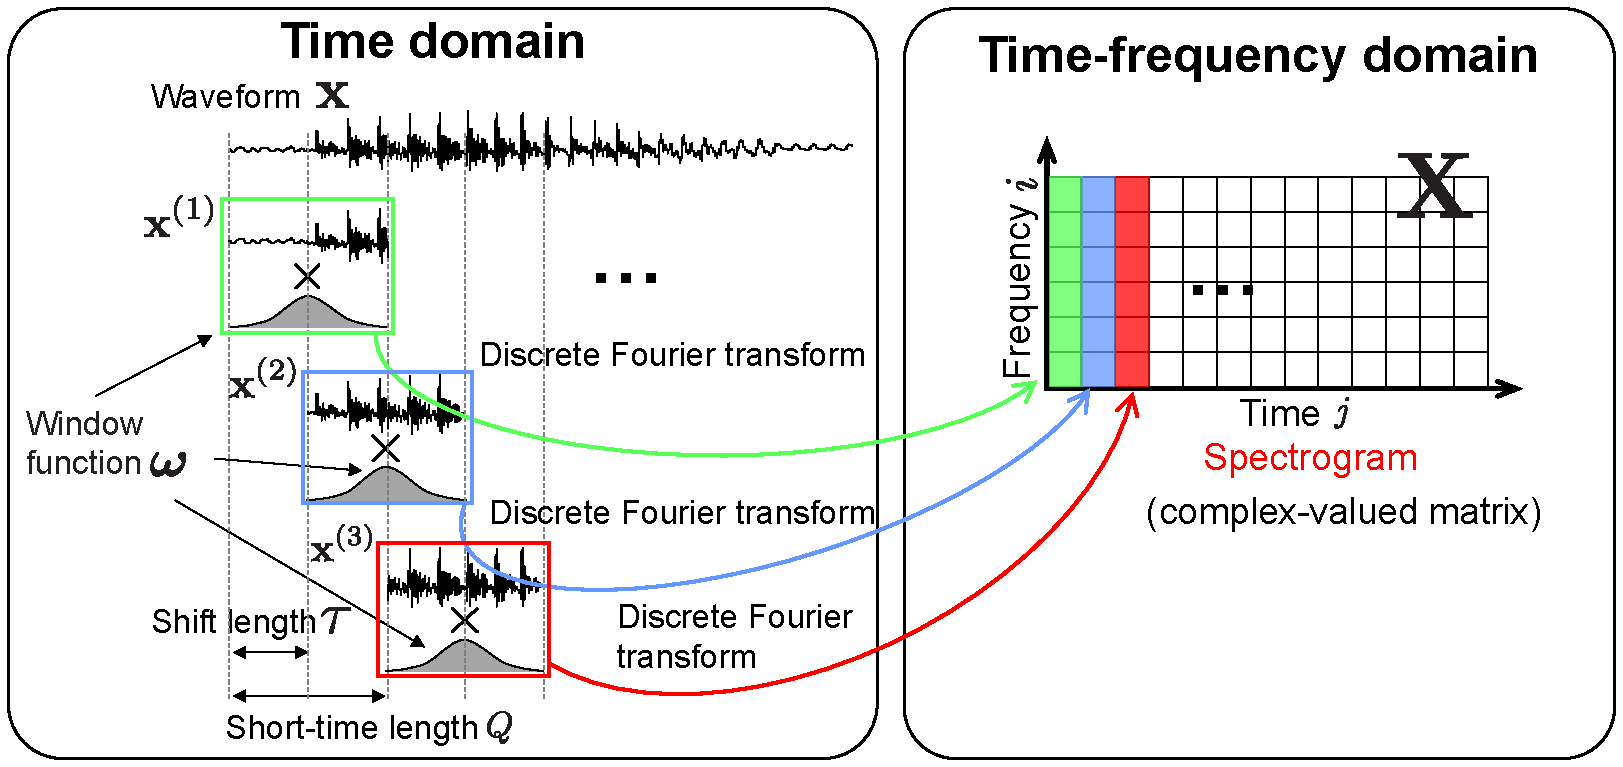
\includegraphics[width=0.95\columnwidth]{figures/stft.pdf}
    \end{center}
    \vspace{-8pt}
	\caption{Mechanism of STFT. Each of windowed short-time signals are transformed to frequency domain by discrete Fourier transform.}
	\label{fig:stft}
\end{figure}
%%%%%%%%%%%%%%%%%%%%%%%%%%%%
STFTはFig.~\ref{fig:stft}に示すような時間的に変化するスペクトルを表現するための手法である.
\red{いま,音響信号の時間波形を次式で定義する.
\begin{align}
  \mathbf{x} = [\mathrm{x}(1), \mathrm{x}(2), \dots, \mathrm{x}(l), \dots, \mathrm{x}(L)]^\mathrm{T} \in \mathbb{R}^L
\end{align}
}
STFT の分析窓関数の長さ及びシフト長をそれぞれ$Q$及び$\tau$としたとき,時間領域の信号
$\cancel{z(l)} \red{\mathbf{x}}$の$j$番目の短時間区間(時間フレーム)の信号は次式で表される.
\begin{align}
    \bm{\cancel{z} \red{\mathbf{x}}}^{(j)} &= \left[\cancel{z} \red{\mathrm{x}}\left((j-1)\tau+1\right), \cancel{z} \red{\mathrm{x}}\left((j-1)\tau+2\right), \cdots , \cancel{z} \red{\mathrm{x}}\left((j-1)\tau+Q\right) \right]^{\cancel{T} \red{\mathrm{T}}}\\
    &= \left[
    \cancel{z} \red{\mathrm{x}}^{(j)}(1),\cancel{z} \red{\mathrm{x}}^{(j)}(2),\cdots , \cancel{z} \red{\mathrm{x}}^{(j)}(q), \cdots , \cancel{z} \red{\mathrm{x}}^{(j)}(Q)
    \right]^{\cancel{T} \red{\mathrm{T}}}~\in \mathbb{R}^{Q}
\end{align}
ここで,$j= 1, 2, \cdots , J$及び$q= 1, 2, \cdots , Q$は,それぞれ時間フレーム及び時間フレーム内のサン
プルを示す.また,セグメント数$J$は次式によって与えられる.
\begin{align}
    J = \frac{L}{\tau}
\end{align}
\blue{また,各時間フレームの信号のSTFTは次式のようにして求められる.}
\red{ただし,時間領域の信号$\mathbf{x}$は式(2.18)が自然数となるように,信号の末尾に必要な分だけ零値が追加されているものとする.このとき,信号$\mathbf{x}$のSTFTを次式で表す.}
\begin{align}
\cancel{\bm{Z}} \red{\mathbf{X}}= {\rm STFT}_{\bm{\omega}}(\cancel{\bm{z}} \red{\mathbf{x}})~\in \mathbb{C}^{I \times J}
\end{align}
\blue{スペクトログラム{$\bm{Z}$}の}\red{ここで,$\mathbf{X}$は(複素)スペクトログラムと呼ばれ,Fig.~\ref{fig:stft}に示すように時間と周波数の2次元の行列である.スペクトログラム$\mathbf{X}$の}$(i, j)$ 番目の要素は次式で表される.
\begin{align}
    \cancel{z} \red{\mathrm{x}}_{ij}= \sum_{q=1}^{Q}\omega(q) \cancel{z}\red{\mathrm{x}}^{(j)}(q){\rm exp}\left\{\frac{-\iota2\pi(q-1)(i-1)}{F}\right\}
\end{align}
ここで$F$は$\lfloor \frac{F}{2}\rfloor+1 =I$を満たす整数($\lfloor \cdot \rfloor$は床関数)\blue{を},$i= 1, 2, \cdots , I$は周波数ビンのインデクス\blue{を},
$\iota$は虚数単位\blue{を},\cancel{$\bm{\omega}$}\red{$\bm{\omega} = [ \omega(1), \omega(2), \dots, \omega(Q) ]^\mathrm{T} \in \mathbb{R}^{Q}$}は\blue{分析窓関数}\red{短時間信号$\mathbf{x}^{(j)}$の両端の不連続性を解消するための解析窓関数}を\red{それぞれ}示している.
このように\red{STFTは,}時間領域の信号は一定幅\blue{短時間ごとに分析窓関数を乗じて離散フーリエ変換を行うことで,}\red{短時間信号に分割して解析窓関数を乗じて離散フーリエ変換を適用し,}\blue{横軸が時間,縦軸が周波数の}スペクトログラムと呼ばれる\blue{複素行列}\red{複素時間周波数行列}\cancel{$\bm{Z}$}\blue{で表すことができる.}\red{に変換する処理である.音源分離等の多くの音響信号処理では,このスペクトログラムを信号処理の対象とする.}


%----------------------------------------------
\section{周波数領域におけるBSSの定式化}
\label{sec:formularization}
%----------------------------------------------
\blue{今一度}\red{本節以降},音源数と観測チャネル数(マイクロホン数)をそれぞれ$N$及び$M$とする.
また,\blue{各観測音源信号をSTFTすることで得られる,各時間周波数における音声信号,} \blue{混合信号,及び分離信号をそれぞれ} \red{音源信号,観測信号,及び分離信号の時間周波数毎の成分をそれぞれ次式で表す.}
\begin{align}
  \bm{s}_{ij} &= \left[
	s_{ij\cancel{,1}\red{1}},s_{ij\cancel{,2}\red{2}}, \cdots, s_{ij\cancel{,n}\red{n}}, \cdots, s_{ij\cancel{,N}\red{N}} 
  \right]^\mathrm{T}~\in \mathbb{C}^{N} \label{f:BSS_s}\\
  \bm{x}_{ij} &= \left[
      x_{ij\cancel{,1}\red{1}},x_{ij\cancel{,2}\red{2}},  \cdots, x_{ij\cancel{,m}\red{m}}, \cdots  , x_{ij\cancel{,M}\red{M}} 
  \right]^\mathrm{T}~\in \mathbb{C}^{M}  \label{f:BSS_x}\\
  \bm{z}_{ij} &= \left[
      z_{ij\cancel{,1}\red{1}},z_{ij\cancel{,2}\red{2}},  \cdots, z_{ij\cancel{,n}\red{n}}, \cdots  , z_{ij\cancel{,N}\red{N}} 
  \right]^\mathrm{T}~\in \mathbb{C}^{N} \label{f:BSS_z}
\end{align}

\blue{と表す.}

\blue{また,複素スペクトログラム行列 {\cancel{$\bm{S}_{n} \in \mathbb{C}^{I\times J}$, $\bm{X}_{m} \in \mathbb{C}^{I\times J}$}}} \cancel{$\bm{Z}_{n} \in \mathbb{C}^{I\times J}$} \blue{の成分をそれぞれ
} \cancel{$s_{i, j, n}$, $x_{i, j, m}$} \blue{及び{\cancel{$z_{i, j, n}$}} と表す.}
\red{式(\ref{f:BSS_s})--(\ref{f:BSS_z})はいずれも複数音源又は複数チャネルをまとめたベクトルであるが,音源又はチャネルではなく時間周波数でまとめた行列も定義しておく.即ち,$n$番目の音源信号のスペクトログラム,
$m$番目の観測信号のスペクトログラム,及び$n$番目の分離信号のスペクトログラムをそれぞれ$\bm{S}_n\in\mathbb{C}^{I\times J}$,$\bm{X}_m\in\mathbb{C}^{I\times J}$,及び$\bm{Z}_n\in\mathbb{C}^{I\times J}$と定義する.これらの行列の$(i,j)$番目の要素はそれぞれ$s_{ijn}$,$x_{ijm}$,及び$z_{ijn}$に一致する.}

%----------------------------------------------
\section{FDICA}
\label{sec:fdica}
%----------------------------------------------
\ref{sec:ica}節で説明したように,ICAとは,観測信号が独立信号の線形結合として観測される場合に,各信号間の独立性を最も高めるよう\blue{に線形分離行列}\red{な分離行列}を推定することでBSSを実現する手法である.
\blue{実際に観測される音声信号には残響の影響を受けており}\red{実際の音響信号の混合は収録環境の残響の影響を受けるため},\blue{線形時不変な}\red{各音源から各マイクロホンまでの空間伝達系の}インパルス応答が畳み込まれて混合される.
インパルス応答の畳み込みは残響長$R$を用いて次式のように表される.
\begin{align}
  \cancel{\bm{x}(l)}\red{\tilde{\bm{x}} (l)} = \sum_n \sum_{l^{'}=0}^{R-1} \tilde{\bm{a}}_n(l^{'}) \cancel{\bm{s}_n(l-l')} \red{\tilde{s}_n (l - l')}
  \label{f:tatami}
\end{align}
ここで\red{,$\tilde{\bm{x}}(l)=[ \tilde{x}_1(l), \tilde{x}_2(l), \cdots, \tilde{x}_M(l) ]^\mathrm{T}$及び$\tilde{s}_n(l)$はそれぞれ時間領域の観測信号及び($n$番目の)音源信号であり},$\tilde{\bm{a}}_n(l)$は\blue{,}音源{$n$}に対する畳み込み混合係数ベクトル(\blue{音源{$n$}からマイクロフォン{$m$}}\red{$n$番目の音源から全マイクロホン}までのインパルス応答を\blue{まとめたもの}\red{時間$l$毎にまとめたもの})である.
\blue{これを}\red{式(\ref{f:tatami})のように混合される複数の音源を}分離するためには\red{,分離行列ではなく}逆畳み込みフィルタを推定することが必要となる.
一般的に逆畳み込みフィルタの推定\blue{は容易ではないことから}\red{非常に困難な問題となってしまうことから},時間領域でのICAによるBSSは\blue{困難である}\red{容易ではない}.
この問題を解決するために,\blue{式({\ref{f:tatami}})}\red{各信号のSTFTによる時間周波数表現を用いて,式(\ref{f:tatami})}の時間領域における畳み込み混合を,\blue{STFTによって}\blue{周波数領域上での}\red{時間周波数領域での周波数毎の}瞬時混合に変換し,時間周波数領域で周波数毎にICAを行うFDICAが提案された\red{~\cite{FDICA}}.

FDICAでは,周波数毎の時不変な混合行列 \cancel{$\bm{A}_{i} = (\bm{a}_{i, 1} ~\bm{a}_{i, 2} ~\cdots ~\bm{a}_{i, n}~\cdots,\bm{a}_{i, N} )\in \mathbb{C}^{M\times N}$}\red{$\bm{A}_{i} = [\bm{a}_{i1} ~\bm{a}_{i2} ~\cdots ~\bm{a}_{in}~\cdots,\bm{a}_{iN} ]\in \mathbb{C}^{M\times N}$}を定義し,混合信号が次式で表現できると仮定する.
\begin{align}
 \bm{x}_{ij} = \bm{A}_i\bm{s}_{ij}
\end{align}
この混合モデルは,\blue{STFTの窓長が室内残響よりも長い場合にのみ成立}\red{観測信号収録時の残響長よりもSTFTの短時間区間長$Q$が十分長い場合に成立}する.
以後,決定的な系($M=N$)を仮定すると,混合行列$\bm{A}_{i}$が正則であれば,\blue{分離行列}\red{周波数毎の分離行列}\cancel{$\bm{W}_i=\bm{A}_i^{-1}=(\bm{w}_{i,1}~\bm{w}_{i,2}~ ...~ \bm{w}_{i, n}~ ... ~\bm{w}_{i, N})^{\mathrm{H}}$}\red{$\bm{W}_i=\bm{A}_i^{-1}=[\bm{w}_{i1}~\bm{w}_{i2}~ ...~ \bm{w}_{in}~ ... ~\bm{w}_{iN}]^{\mathrm{H}}$}を用いて,分離信号を次式で表せる.
\begin{align}
 \bm{z}_{ij} = \bm{W}_{i}\bm{x}_{ij} \label{eq:sep}
\end{align}
ここで,$\cdot^\mathrm{H}$はベクトルや行列のエルミート転置を示す.
分離行列の行ベクトルである$\bm{w}_{i,n}\in\mathbb{C}^M$は,\blue{周波数{$i$}}\red{$i$番目の周波数ビン}において,観測信号から$n$番目のみの\blue{音源}\red{音源が含まれる分離信号}へ変換する分離フィルタである.
このようにFDICAでは,観測信号$\bm{x}_{ij}$の各周波数ビンに対しそれぞれ独立に\blue{ICA}\red{(複素数の)ICA}を適用することで,周波数毎の分離行列$\bm{W}_{i}$を全周波数にわたって推定\blue{することで音源分離を行う}\red{し,BSSの達成を目指す}.

%----------------------------------------------
\section{パーミュテーション問題とその解決}
\label{sec:pp}
%----------------------------------------------
FDICA中で周波数毎に適用しているICAは,
\blue{音源間の統計的独立性のみに基づいて分離行列を推定するため} 
\red{\ref{subsec:ica_voluntariness}項で述べた通り},
\blue{分離音源} 
\red{分離された推定信号}の周波数毎のスケール及び順番に関しては不定である.
従って,FDICAの推定分離行列を$\hat{\bm{W}}_i$とすると,次式のような不定性が残る.
\begin{align}
	\hat{\bm{W}}_{i} &= \bm{D}_{i}\bm{P}_{i}  \bm{W}_{i} \label{eq:w_fdica}
\end{align}
ここで,$\bm{P}_i \in \{0, 1\}^{N \times N}$は分離行列$\bm{W}_{i}$の行ベクトル$\bm{w}_{i\cancel{,} n}$の順番を入れ変えうるパーミュテーション行列(置換行列)である.
$\bm{D}_i \in \mathbb{R}^{N \times N}$は,$\bm{w}_{i\cancel{,}n}$のスケールを変化させる可能性のある対角行列である.
即ち,FDICAで推定される分離信号
\begin{align}
\bm{y}_{ij} &= \hat{\bm{W}}_i\bm{x}_{ij} \\
&=\left[ y_{ij\cancel{,}1},y_{ij\cancel{,}2}, \cdots, y_{ij\cancel{,}n}, \cdots, y_{ij\cancel{,}N} \right]^\mathrm{T}~\in \mathbb{C}^{N} \label{eq:sepSig}
\end{align}
は,推定音源の順番やスケールが周波数毎にばらばらになっている状態である.
このうち,$\bm{D}_i$によって生じるスケールの任意性は,\blue{プロジェクションバック法}\red{時間領域でのICAの場合と同様にプロジェクションバック法}\cite{Matsuoka2001_PB}で復元可能である.
一方で,$\bm{P}_i$によって生じる分離信号の順番の任意性(パーミュテーション)を\blue{純粋に}\red{$I$個の全周波数ビンに関して}復元することは,組み合わせ爆発が\blue{発生するため}\red{生じるため}容易ではない.
\red{具体的には,$I$個の周波数ビンのそれぞれで$N$個の音源の順番は$N!$種類あるため,全周波数のパーミュテーションは$(N!)^I$通り存在することになり,その内の正解(全周波数で同一の音源パーミュテーションとなるもの)は$N!$個である.}
この問題は,一般的にパーミュテーション問題と呼ばれる.
パーミュテーション問題の概要をFig.~\ref{fig:permu}に示す.
ここで,FDICAで\blue{推定される分離}\red{得られる推定}信号$\bm{y}_{ij}$の\blue{音源毎の複素スペクトログラム行列を}\red{$n$番目のスペクトログラムを}$\bm{Y}_n \in \mathbb{C}^{I \times J}$\blue{で表している}\red{と定義している}.
FDICA直後の$\bm{Y}_n$に注目すると,周波数毎での音源分離は達成できている.
しかし,時間周波数構造全体としては,異なる\blue{グループ}\red{音源}の\blue{分離信号}\red{分離成分}が1つの\blue{時間周波数構造}\red{時間周波数内}に混在していることが分かる.
これがパーミュテーション問題であり,ICAの分離信号の順番に関する不定性に起因して発生している.
そのため,FDICAにはポスト処理として,分離された音源の順番を全周波数ビンにわたって正しく並べ直す必要がある.
%%%%%%%%%%%%%%%%%%%%%%%%%%%%
\begin{figure}[t]
    \begin{center}
        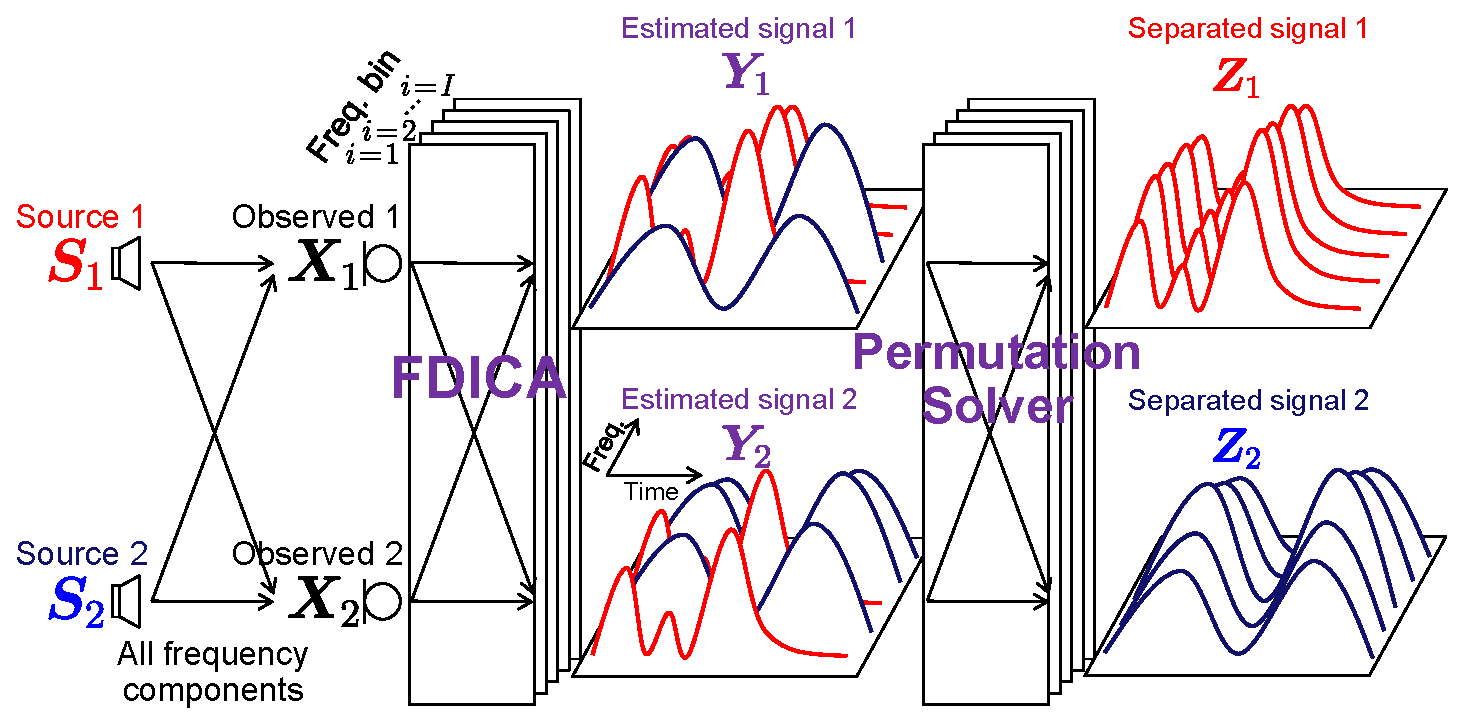
\includegraphics[width=0.95\columnwidth]{figures/permutation_image.eps}
    \end{center}
    \vspace{-8pt}
	\caption{Permutation problem in FDICA, where $N=M=2$.}
	\label{fig:permu}
\end{figure}
%%%%%%%%%%%%%%%%%%%%%%%%%%%%
\blue{パーミュテーション問題を解決して得られる分離信号は次式となる.}\red{このパーミュテーション問題を解決する処理は次式で表される.}
\begin{align}
\bm{z}_{ij} &= \bm{P}_{i}^{-1}\bm{D}_{i}^{-1}\bm{y}_{ij} \label{eq:z}
\end{align}
%本論文では,この$\bm{P}_{i}^{-1}$を推定することが目的となる.
\red{スケールの不定性を補正する$\bm{D}_i^{-1}$はプロジェクションバック法によって解析的に求められる.したがって,パーミュテーション問題の解決とは,全周波数ビンにわたって$\bm{P}^{-1}$を求める問題として解釈できる.}
このパーミュテーション問題を解決するために,これまでにも数々のパーミュテーション解決法が提案されてきた.
代表的な既存手法の1つに,隣接周波数の時系列強度(音源アクティベーション)の相関を用いたパーミュテーション解決法\blue{{\cite{COR}}}\red{~\cite{COR,Permutation_solverBSS}}がある.
これは,\red{Fig.~\ref{fig:permu}に示す赤色と青色の分離信号のように,}分離信号のパーミュテーションが正しければ,隣接した周波数アクティベーション間の相関が高くなりやすいという仮定の下で並べ替える手法である.
\blue{また}\red{このとき},離れた周波数においても,同じ音源のアクティベーション間の相関が高くなるように並び替えられている.
%り,次式のように相関を計算する.
%\begin{align}
%\Tilde{\bm{v}}_{i}(n) &=  \frac{1}{J}\sum_{j=0}^{J} |\bm{y}_{i,j,n}| \\
% {\rm sim}(i) &= \sum_{n\neq m} \frac{\Tilde{\bm{v}}_{i}(n) \cdot \Tilde{\bm{v}}_{i}(m)}{\|
% \Tilde{\bm{v}}_{i}(n)\|~\| \Tilde{\bm{v}}_{i}(m)\|}
%\end{align}
%ここで,$\cdot$は内積を表しており,
他にも,マイクロホンの相対的な位置情報を既知として音源到来方位を計算し,パーミュテーション解決の手掛かりとする手法 \cite{DOA}及び両者を組み合わせたパーミュテーション解決法\red{\cite{DOACOR}}も提案されている.
しかしながら,パーミュテーション問題の解は組み合わせ爆発を起こすことから,上記いずれの手法を用
いても完璧にパーミュテーション問題を解くことは非常に難しく,とくに\blue{複数音声の混合信号}\red{音源数が増加した際}における\red{頑健・}高精度なパーミュテーション問題の解決はいまだ\red{実現}できていない.

%----------------------------------------------
\section{IVAとILRMA}
\label{sec:ivailrma}
%----------------------------------------------
FDICA に対して音源の時間周波数成分の共起関係を新たに仮定して,パーミュテーション問題を回避しつつ分離信号を推定する手法が登場している.
例えば,IVA~\cite{IVA1,IVA2}は,同一音源の周波数成分の共起を仮定しており,
FDICAでは周波数毎に独立性を最大化していたのに対し,IVAでは全周波数成分をまとめてベクトル変数とし,べクトル間の独立性を最大化するようなモデルとなっている.
そのため,\blue{同じ音源の分離信号は全周波数でまとめて出力されるような分離モデルとなっており,} \red{実際に複数の周波数ビンで同時に共起する成分が同一音源としてまとめられるような分離行列が推定され,}パーミュテーション問題を \red{可能な限り}回避することが期待できる.
\red{IVAの「同一音源であれば全周波数が共起する」という仮定は,音源信号の時間周波数構造に関するモデルである.実際に,音声信号はこのような時間周波数構造が比較的適合するため,IVAを用いることである程度パーミュテーション問題を回避できる.}
\blue{また,NMF {~\cite{NMF}}とIVAを組み合わせたBSSであるILRMA~{\cite{ILRMA1,ILRMA2}} は同一源の時周波数成分
の共起が低ランク構造を持つことを仮定しておりIVA と同様にパーミュテーション問題を音源モデルに基づいて可能な限り回避するようなモデルとなっている.}
 \red{さらに,IVAの音源信号の時間周波数構造に関するモデル(以後,音源モデルと呼ぶ)をより詳細なモデルに発展させたBSSとして,ILRMA~\cite{ILRMA1,ILRMA2}が提案されている.ILRMAは,IVAで提案された音源モデルにNMF~\cite{NMF}を用いている.NMFは時間周波数構造を低ランク近似できることから,
「同一音源であれば時間周波数構造は低ランク行列になる」という仮定を考えている.このような音源モデルは音声信号だけでなく音楽信号にもよく適合することから,ILRMAの登場によって多くの場合においてIVAよりも高品質なBSSを達成することができるようになった.}

%%%%%%%%%%%%%%%%%%%%%%%%%%%%
\begin{figure}[t]
  \begin{center}
      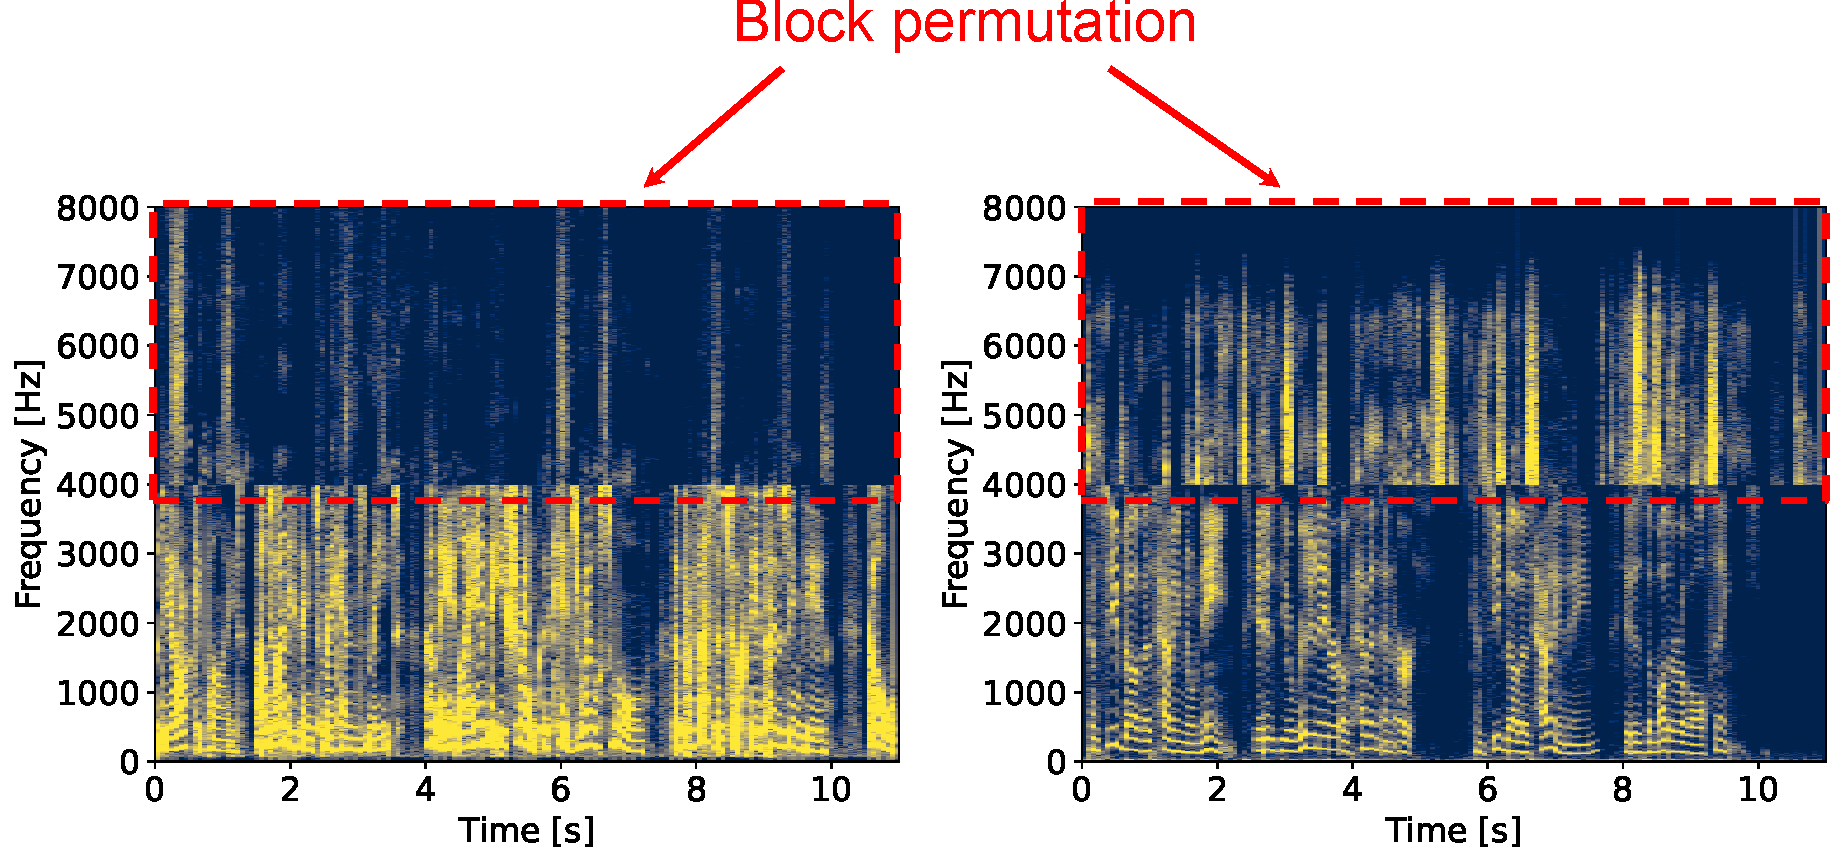
\includegraphics[width=1.00\columnwidth]{figures/block_permu.pdf}
  \end{center}
  \vspace{-8pt}
\caption{Example of block permutation problem.}
\label{fig:bp}
\end{figure}
%%%%%%%%%%%%%%%%%%%%%%%%%%%%

しかし,\blue{音声と音声の混合信号の様な分離タスクの場合,}\red{声質の近い複数音声の混合や,音源数が$N\geq 4$となる過酷な条件においては,}IVAやILRMAを用いてもしばしば分離に失敗してしまう.
これは,\blue{音声信号}\red{各音源信号}の時間周波数成分がダイナミックに変動することから,\blue{音声信号のパワースペクトログラムを低ランクで表現することが難しいことが原因と予想される.}
\red{IVAやILRMAが仮定する音源モデルが同一音源の時間周波数成分を正しく捉えられないことに起因していると思われる.}
\blue{また}\red{例えば},IVAやILRMAにおいて\blue{も},まとまった周波数帯域でパーミュテーションが入れ替わる問題(ブロックパーミュテーション問題)\cite{brock_p}が報告されている.
Fig.~\ref{fig:bp}にブロックパーミュテーション問題の様子を示す.
Fig.~\ref{fig:bp}では,\blue{{$4000$hz}}\red{4~kHz}以上の周波数帯が\blue{まとめて反転していることが分かる.}\red{まとまって入れ替わった状態で分離信号が推定されてしまっている.}
\blue{そのため,}\red{このような事実からも,}依然としてパーミュテーション問題の解決が不十分であることが分かる.
\red{Fig.~\ref{fig:bp}のような明らかなブロックパーミュテーションであれば,ユーザアノテーションにより修正するようなインタラクティブなBSSアルゴリズム\cite{User_anotation}も適用可能であるが,
多くの帯域にブロックパーミュテーション問題が発生する場合もあり,ユーザアノテーションの利用も難しい状況が存在する.}

%----------------------------------------------
\section{深層パーミュテーション解決法}
\label{sec:DNNs}
%----------------------------------------------

\blue{近年では,DNNを用いたパーミュテーション問題解決法が登場している.観測された混合信号{$\bm{X}_n$}にFDICA適用すると,パーミュテーション問題が生じた分離信号{$\bm{Y}_n$}が得られる.
これらのパワースペクトログラム{$|\bm{Y}_n|^{.2}$}から全周波数帯域中の局所的な狭帯域(サブバンド)を定義し,サブバンド毎にデータをDNNに入力し,パーミュテーション問題を解決する.
サブバンド毎に参照周波数を定義し,その近傍周波数が参照周波数に対して同一音源か否かを判断し,同一音源である場合はDNNの出力として「0」を出力し,同一音源でない場合はDNNの出力として「1」を出力する.
この結果を時間方向にずらして,全時間フレームに対するDNNの予測処理を走査する.そして,DNNの予測結果を時間方向に対して多数決処理を行うことで,より信頼性の高いサブバンドベクトルを取得する.
サブバンドベクトルは,基準周波数{$i$}をシフトすることにより全周波数を推定する.ただ,各サブバンドベクトル内の2値は(「0」及び「1」)は異なる意味を持つ可能性がある.これはサブバンド内の周波数成分が.
参照周波数の成分と同一音源か否かを示しているに過ぎず,参照周波数の変化を共に,対応音源が変化する.2音源の場合を考えるとサブバンドベクトル内の値が「1」,つまり同一音源ではない時,必然的にもう一方の音源を指すこととなる.
但し,3音源以上になるとサブバンドベクトル内の値が「1」の時,残りのどの音源のことを指すのかが判断できない.
3音源以上になると組み合せ爆発を起こしてしまい,計算量の観点から3音源以上の音源分離は難しい.}

\red{前節で述べた通り,IVAやILRMAのように音源モデルを仮定してパーミュテーション問題を回避する方法は頑健性や汎化性という観点で課題が残る.
観測信号中に混合している各音源信号の時間周波数構造に合致した適切な音源モデルが仮定できれば高性能となる反面,合致しなければブロックパーミュテーション問題を引き起こしてしまう.}

\red{この問題を解決するために,様々な種類の音源のデータからパーミュテーション問題を解決する最適なモデルを学習するアプローチ(深層パーミュテーション解決法)が近年提案された\cite{DNN_soluver}.
この手法では,学習データのパーミュテーション問題を解くDNNを構築することで,あらゆる種類の観測信号に対しても高精度にパーミュテーション問題を解くことを目指している.
但し,全周波数ビンを一度に取り扱いパーミュテーション問題を解くことはDNNを用いてもなお困難であったため,前段で一定幅の周波数帯域(サブバンド)内のパーミュテーション問題の解決を様々なサブバンドに適用し,
後段でサブバンド間のパーミュテーション問題をスティッチング\cite{stiching}により解決するという複雑な二段階処理のアルゴリズムとなっている.
さらに,前段のサブバンド内のパーミュテーション解決さえも困難であったことから,「参照周波数ビンとその他の周波数ビンの推定信号成分が同一音源か否か」という2値分類DNNを学習しており,
音源数が$N\geq 3$の場合は後段のサブバンド間のスティッチングが非常に複雑・煩雑なアルゴリズムとなってしまう問題をはらんでいる.
そのため,文献~\cite{DNN_soluver}の深層パーミュテーション解決法は$N=2$の場合を想定しており,一般的なBSSへの応用は難しい.}

\red{しかしながら,DNNに基づくパーミュテーション問題の解決というアプローチは,前述の通り多様な音源信号に対して適用できる可能性があるという観点で深い意義がある.
本論文においても,次章の動機で述べる通り,深層パーミュテーション解決法の可能性を基礎実験的に調査し,その有用性について検証する.}


%----------------------------------------------
\section{本章のまとめ}
\label{sec:conclu}
%----------------------------------------------
本章では,提案手法において必要となる基礎理論及び各種従来手法について説明した.
\red{\ref{sec:ica}節では,ICAの基本原理と分離信号における順序とスケールの任意性について説明した.
\ref{sec:stft}節では,音響信号処理でよく用いられる手法であるSTFTについて説明した.
\ref{sec:formularization}節では,各信号の成分を時間周波数毎に定式化を行い,\ref{sec:fdica}節以降で用いる.
\ref{sec:fdica}節では,時間周波数領域での周波数毎にICAを適用することで音源分離を行うFDICAについて説明した.
\ref{sec:pp}節では,FDICAに伴い生じるパーミュテーション問題について説明した.
\ref{sec:ivailrma}節では,パーミュテーション問題を可能な限り回避するような手法である,IVAとILRMAについて説明した.}
次章以降では,より簡潔に精度の良いBSSを達成するために\ref{sec:fdica}節で導入したFDICAのポスト処理として,DNNに基づくパーミュテーション解決法を新たに提案する.
















